%----------------------------------------------------------------------------------------
%	PACKAGES AND DOCUMENT CONFIGURATIONS
%----------------------------------------------------------------------------------------

\documentclass{article}

\usepackage[version=3]{mhchem} % Package for chemical equation typesetting
\usepackage{siunitx} % Provides the \SI{}{} and \si{} command for typesetting SI units
\usepackage{graphicx} % Required for the inclusion of images
\usepackage{natbib} % Required to change bibliography style to APA
\usepackage{amsmath} % Required for some math elements 
\usepackage[utf8x]{inputenc} 

\setlength\parindent{0pt} % Removes all indentation from paragraphs

\renewcommand{\labelenumi}{\alph{enumi}.} % Make numbering in the enumerate environment by letter rather than number (e.g. section 6)

%\usepackage{times} % Uncomment to use the Times New Roman font

%----------------------------------------------------------------------------------------
%	DOCUMENT INFORMATION
%----------------------------------------------------------------------------------------

\title{Deterministic and Heur arpproach \\ on finding the minimum of a function} % Title

\author{Andrei \textsc{Ianău}} % Author name

\date{\today} % Date for the report

\begin{document}

\maketitle % Insert the title, author and date

\begin{center}
\begin{tabular}{l r}
Date Performed: & \date{10/10/2019} \\ % Date the experiment was performed
Professor: & Croitoru Eugen % Instructor/supervisor
\end{tabular}
\end{center}


%----------------------------------------------------------------------------------------
%	ABSTRACT
%----------------------------------------------------------------------------------------

\begin{abstract}

The importance of a genetic algorithm is beyond comprehension. Not only that we have impossbile problems to solve by human intelligence, but we have discovered a way on how to have a chance against the most complicated questions in the universe, \emph{genetic-algorithms}. 
Indeed, this is not enough, for we, humans, are forever in the search of excelence and that is why there exist communities of scientists that try to create better and better algorithms that can solve problems.

\end{abstract}

%----------------------------------------------------------------------------------------
%	SECTION 1
%----------------------------------------------------------------------------------------

\section{Objective}

Find the difference between a deterministic algorithm and a non-deterministic algorithm that has 94\% chance on discovering the root of 4 functions:
\begin{enumerate}
	\item Booth
	\item Eusom
	\item Shubert
	\item Rastrigin
\end{enumerate}

% If you have more than one objective, uncomment the below:
%\begin{description}
%\item[First Objective] \hfill \\
%Objective 1 text
%\item[Second Objective] \hfill \\
%Objective 2 text
%\end{description}

\subsection{Definitions}
\label{definitions}
\begin{description}
\item[Booth Function]

\begin{equation}
f(X)=\left(x_1+2x_2-7\right)^2+\left(2x_1+x_2-5\right)^2
\end{equation}

\item[Eusom Function]

\begin{equation}
f(x,y)=−cos(x_1)cos(x_2) exp(−(x − \pi)^2−(y − \pi)^2)
\end{equation}

\item[Shubert Function]

\begin{equation}
f(\mathbf{x})=f(x_1, ...,x_n)=\prod_{i=1}^{n}{\left(\sum_{j=1}^5{ cos((j+1)x_i+j)}\right)}
\end{equation}

\item[Rastrigin Function]

\begin{equation}
f(x, y)=10n + \sum_{i=1}^{n}(x_i^2 - 10cos(2\pi x_i))
\end{equation}

\end{description} 
 
%----------------------------------------------------------------------------------------
%	SECTION 2
%----------------------------------------------------------------------------------------

\section{Setup}

	The language that tha algorith is written is \emph{C++} to improve the speed.
Simple data structure were used: simple variables, matrixes.\par

	The experiments are done within 2, 5 and 20 dimensions vectors. 
For each dimension, each function will be ran with a deterministic or non-deterministic aproach to find the minimum.
The non-deterministic aproach will be composed of 5000 runs of a random input and taken the minimum from all of these 5000 runs.
Each non-deterministic experiment will be ran 3000 times to create a statistic that can showcase the probability/the chances of that aproach.


%----------------------------------------------------------------------------------------
%	SECTION 3
%----------------------------------------------------------------------------------------

\section{Sample Calculation}

\begin{center}
 \begin{tabular}{||c || c | c | c | c ||} 
 \hline
 Functions & Booth & Easom & Shubert & Rastrigin \\
 \hline
 Determ & 10  & -0.000030 & 0.989725  & 5 \\ 
 \hline
 Min Heur & 1e-05 & -0.998634 & -84.80898 & 0 \\
 \hline
 Mean Heur & 0.00370408 & -0.8463373 & -84.75004 & 0.0530826 \\
 \hline
 StdDev Heur & 0.003893287 & 0.1331897 & 0.06020627 & 0.06103807 \\
 \hline
\end{tabular}
\end{center}



\begin{figure}[h!]
    \centering
    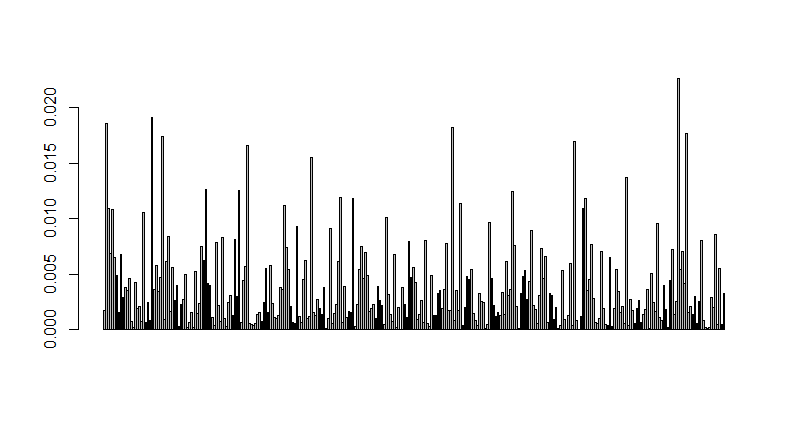
\includegraphics[width=1\textwidth]{./results/booth2}
    \caption{Booth in 2 dimensions}
    \label{fig:Booth in 2 dimensions}
\end{figure}

\begin{figure}[h!]
    \centering
    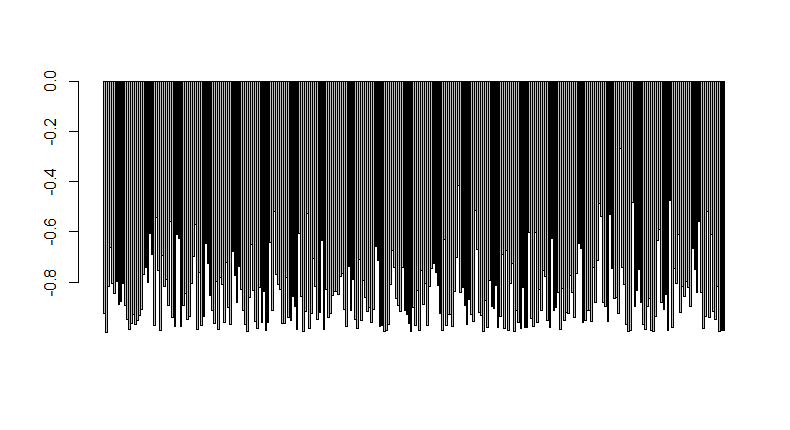
\includegraphics[width=1\textwidth]{./results/Easom2}
    \caption{Easom in 2 dimensions}
    \label{fig:Easom in 2 dimensions}
\end{figure}

\begin{figure}[h!]
    \centering
    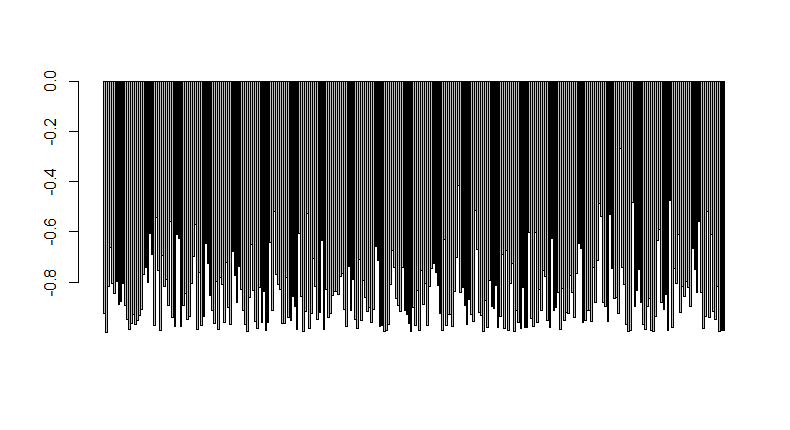
\includegraphics[width=1\textwidth]{./results/Easom5}
    \caption{Easom in 5 dimensions}
    \label{fig:Easom in 5 dimensions}
\end{figure}

\begin{figure}[h!]
    \centering
    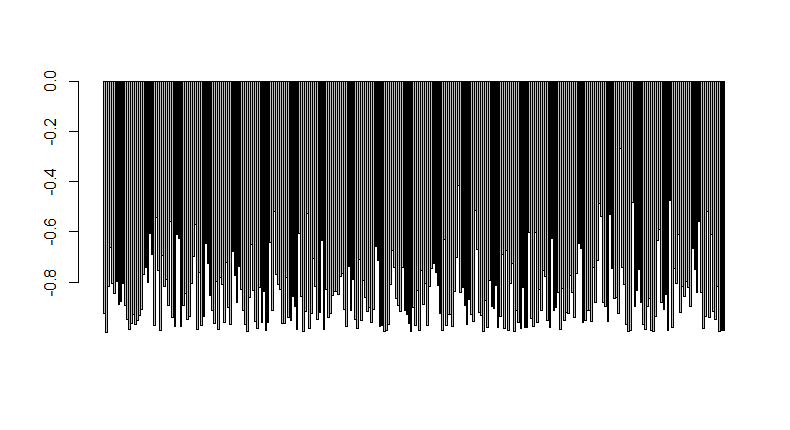
\includegraphics[width=1\textwidth]{./results/Easom20}
    \caption{Easom in 20 dimensions}
    \label{fig:Easom in 20 dimensions}
\end{figure}

\begin{figure}[h!]
    \centering
    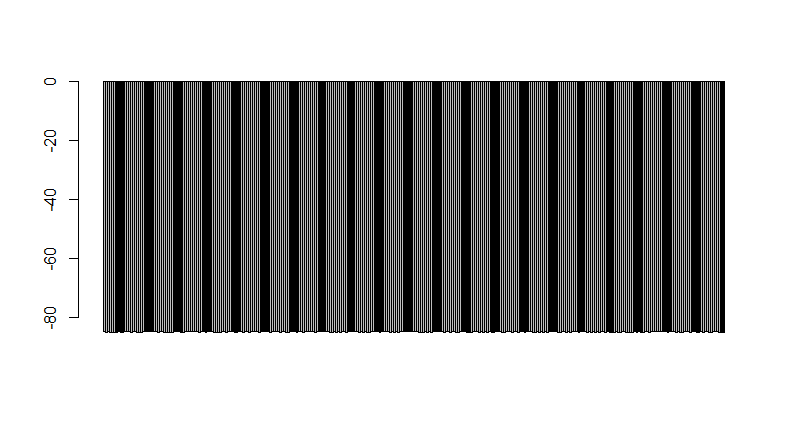
\includegraphics[width=1\textwidth]{./results/Shubert2}
    \caption{Shubert in 2 dimensions}
    \label{fig:Shubert in 2 dimensions}
\end{figure}

\begin{figure}[h!]
    \centering
    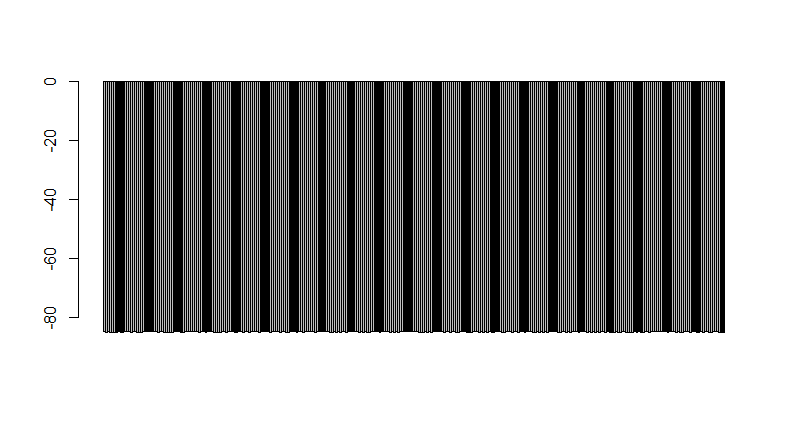
\includegraphics[width=1\textwidth]{./results/Shubert5}
    \caption{Shubert in 5 dimensions}
    \label{fig:Shubert in 5 dimensions}
\end{figure}

\begin{figure}[h!]
    \centering
    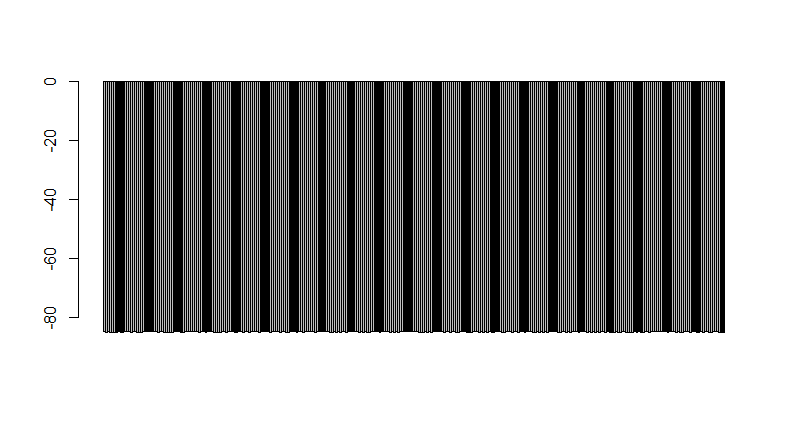
\includegraphics[width=1\textwidth]{./results/Shubert20}
    \caption{Shubert in 20 dimensions}
    \label{fig:Shubert in 20 dimensions}
\end{figure}

\begin{figure}[h!]
    \centering
    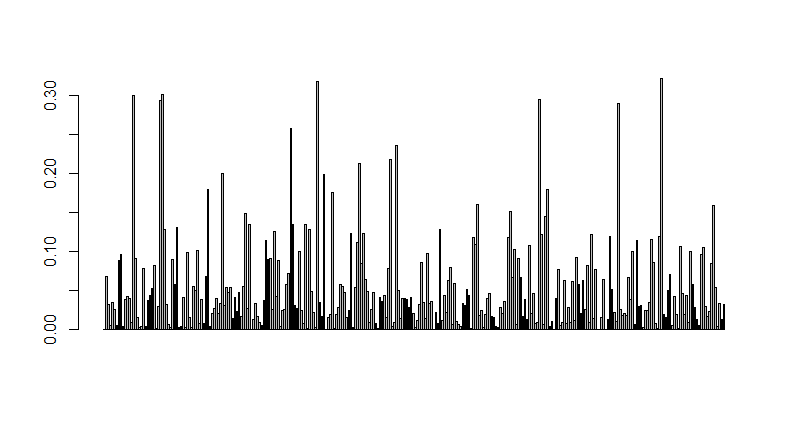
\includegraphics[width=1\textwidth]{./results/Rastrigin2}
    \caption{Rastrigin in 2 dimensions}
    \label{fig:Rastrigin in 2 dimensions}
\end{figure}

\begin{figure}[h!]
    \centering
    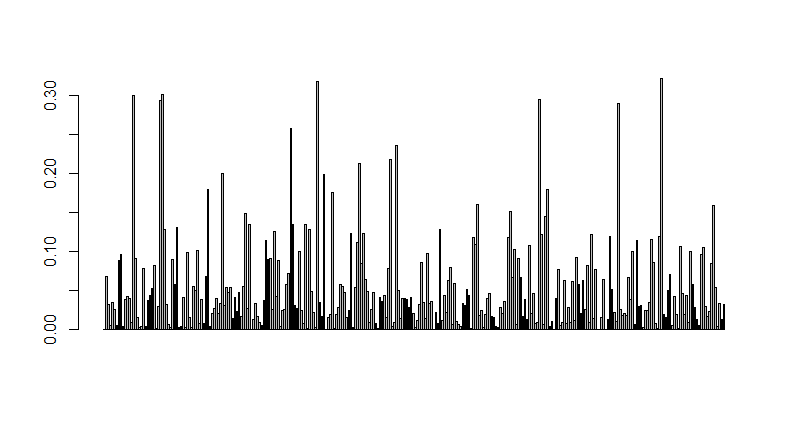
\includegraphics[width=1\textwidth]{./results/Rastrigin5}
    \caption{Rastrigin in 5 dimensions}
    \label{fig:Rastrigin in 5 dimensions}
\end{figure}

\begin{figure}[h!]
    \centering
    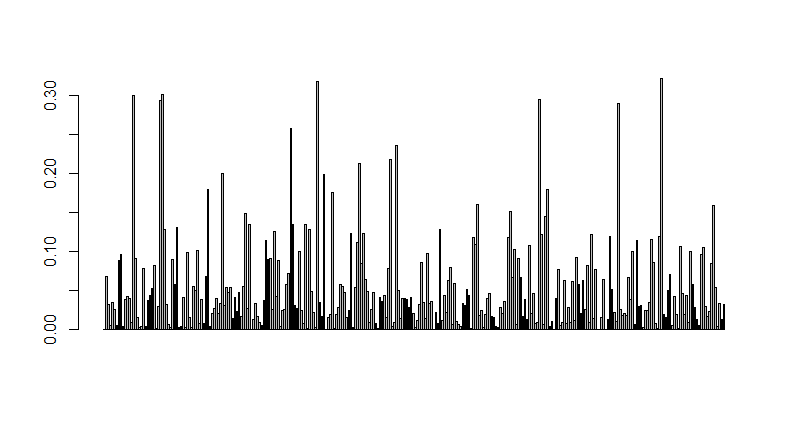
\includegraphics[width=1\textwidth]{./results/Rastrigin20}
    \caption{Rastrigin in 20 dimensions}
    \label{fig:Rastrigin in 20 dimensions}
\end{figure}



%----------------------------------------------------------------------------------------
%	SECTION 4
%----------------------------------------------------------------------------------------


\section{Conclusion}
The fact that we can get this good only with a random search algorithm demonstrates the power of randomness.
The true power within these algorithms resides in their capability to transform themselves in better versions. 
This is so called "genetic-algorithm" that can determine the desired solution to a problem that no deterministic algorithm can provide in polynomial time.


\end{document}